\documentclass{article}


\usepackage{arxiv}
\usepackage{setspace}
\usepackage[utf8]{inputenc} % allow utf-8 input
\usepackage[T1]{fontenc}    % use 8-bit T1 fonts
\usepackage{hyperref}       % hyperlinks
\usepackage{url}            % simple URL typesetting
\usepackage{booktabs}       % professional-quality tables
\usepackage{amsfonts}       % blackboard math symbols
\usepackage{nicefrac}       % compact symbols for 1/2, etc.
\usepackage{microtype}      % microtypography
\usepackage{lipsum}
\usepackage{graphicx}
\graphicspath{ {./images/} }

\doublespacing

\title{Generative Adversarial Networks for PCG Arrhythmia Detection}


\author{
 Aditya Kendre \\
  Cumberland Valley High School\\
  Mechanicsburg, PA 17050 \\
}

\begin{document}
\maketitle
\begin{abstract}
With the rapid growth of computational power and complex algorithms, we propose a novel approach to detect arrhythmias in Phonocardiograms (PCGs). Typically, Electrocardiograms are used to diagnose arrhythmias; requiring medical grade equipment to accurately recognize cardiac illnesses (Rajpurkar et al., 2017). PCGs, however, provide ease of access to everyone who has a device capable of recording audio, allowing medical professionals to treat arrhythmias in the developmental stages. The new design comprises two subsystems; one is based on the relationship between Electrocardiograms (ECGs) and PCGs, and the other between PCGs and arrhythmias. The association between ECGs and PCGs is amended to translate from one space to another, where ECGs become dimensionally reduced, then reconstructed into a PCG signal. The second subsystem uses a Generative Adversarial Networks (GAN), in which both arbitrary PCG signals are generated, and preexisting ECG datasets are recreated into PCG signals (using subsystem one). These signals are fed into a classifier that detects if an arrhythmia is present. This proposed system's advantage is that PCG data is more readily available than ECG data; hence, more heart diagnostics can be made.
\end{abstract}

\section{Introduction}
\paragraph{Problem statement.}
Late diagnosis of cardiac arrhythmias.
\paragraph{Solution.}
Diagnosing arrhythmias with PCG recordings.

Electrocardiograms have created a profound impact in the field of cardiology, specifically in recognizing heart arrhythmias, a problem with the rhythm of one’s heartbeat. Noninvasive arrhythmia analysis is based on multiple electrodes that reflect the electrical activity on ECGs. However, with the recent surge of heart-related medical cases, it is getting difficult to diagnose heart conditions at an early stage. As most treatments rely on detecting the disease in it's infancy stages. Traditionally, arrhythmias are diagnosed by cardiologists by analyzing ECG recordings (Jordaens, 2018). Some clinics have adopted a new technique in which ECG and PCG signals are simultaneously recorded and then computationally analyzed. This, however, still requires an instrument capable of recording ECG data. Such instruments are only available during scheduled appointments, often which are recommended by physicians.
If a physician fails to detect symptoms of arrhythmia, a patient may never receive a diagnosis. One study found 44\% of cardiologists were not able to detect common cardiac events with stethoscopes (Mangione et al., 1993); in another study, delays in cardiac-related illness diagnosis and treatment impacted procedural success rates by as much as 24\% (Bunch et al., 2013). We propose a method where it is now possible to accurately detect arrhythmias with only PCG recordings. This provides an opportunity for physicians to check for potential developments of cardiac arrhythmias at every physical exam accurately.

Current PCG arrhythmia diagnosis methods only recognize between Normal and Abnormal (binary classification), providing minimal information about what is present within the PCG signal (Aziz et al., 2020). This is because no PCG datasets exist that include more than 3 classes of arrhythmia. Therefore, it is necessary to transform pre-existing ECG datasets with multiple classes to PCG signals. This enables models to detect a larger range of arrhythmia without explicitly collecting new PCG recordings. Currently, no technology attempts to construct PCG signals from existing ECG data.

\section{Methodology}

\subsection{Approach}
The model contains two sub-models, an Autoencoder (AE), and a Generative Adversarial Network (GAN). The AE is responsible for extracting relevant features from an ECG signal and constructing a PCG signal from the latent features. The GAN is responsible for extracting relevant features and classifying the PCG signals.

The training phase involves 3 stages: AE training, AE+GAN training, and GAN fine-tuning. During training phases, all datasets will follow the following split: 70\% - training, 15\% - validation, 15\% - testing; this cross-validation step validates that both models are not overfitting during the training phase. The first stage involves training the AE with a supervised dataset of ECG and PCG signals (Liu et al, 2016). The second stage involves training both the AE and the GAN with a supervised dataset of arrhythmias within ECGs (Goldberger et al., 2017). During the training process, the AE model will be frozen (the weights and biases of the AE model won't be trained) as this process is already done in the preceding stage. The last stage is fine-tuning the GAN  on a binary supervised dataset of PCG signals (Normal vs Abnormal). This validates the model's metrics in the previous step.  
\begin{center}
    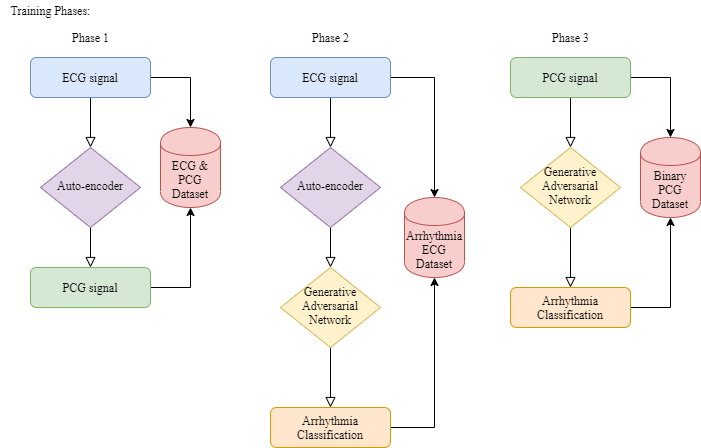
\includegraphics[scale=0.70]{training-digram}
\end{center}

\subsection{Resources}
The majority of the resources and funding needed for this research project involve cloud computing services such as AWS. The service will be running virtual machine instances of TPUs or GPUs. These instances serve to speed up the training process. Additionally, I'm planning on working with Professor Vasant Honavar from Penn State, in addition to experience in Machine Learning, Professor Honavar has published many papers regarding cardiac-diseases.

\subsection{Goals}
While testing and training, the model will be validated against with metrics such as recall, precision, accuracy, loss, FBeta, F1 score, and ROC/AUC score. These tests will ensure that the model is accurately predicting the classes, and identifying important features within the datasets. Each step in the training phase will represent a milestone and an accuracy of 97\% will mark the completion criteria.

\subsection{Risks}
\paragraph{Overfitting:}
One of the largest problems in Deep Learning overall, which possesses a threat to our model is overfitting. Overfitting typically happens when the model metrics of the training and validation set diverge. This suggests that the model is not generalizing, but rather memorizing the training dataset. To combat overfitting, researchers typically implement data argumentation techniques to reinforce important features in a dataset. 

\paragraph{Domain Shift:}
A domain shift occurs when a source dataset performs well but on a different dataset distribution, the performance drastically decreases. Typically, domain adaptation is often used to improve performance on target datasets. This is done by training the model itself on multiple datasets to improve the model's capacity to generalize.

\paragraph{Traning Time:}
With large multi-model architectures, it becomes tough to train models on a single GPU. This can happen for a number of reasons, but the main reason is because the model takes up too much memory of the GPU. Generally, parallel processing is used to split tasks and assign them to different GPUs. For instance, the AE model will run on a single GPU, while the GAN will run on another GPU.

\subsection{Timeline}
Each milestone will be completed on a two-week schedule, starting from February 13th.
Data preprocessing - February 27th.
Training Phase 1 - March 13th.
Training Phase 2 - March 27th.
Training Phase 3 - April 3rd.
Deployment - April 17th.


\subsection{Current Progress}
Although I have not done any work on this particular project, I do hope to gather aid from MIT THINK Scholars: Audrey Cui and Katherine Xiong. They both have experience in computer science in biology and healthcare which I feel will be extremely helpful during the model construction process. Additionally, I wish to use all of the funding from the program for the cloud computing services that I will use to run and train the models.

\subsection{Project Budget}
\begin{tabular}{lllll}
                & Price per Hour & Hours      & Cost   &  \\
NVIDIA A100 GPU & \$3.10         & 225        & 697.50 &  \\
                &                & Total Cost & 697.50 &  \\
                &                &            &        & 
\end{tabular}

\section{Background}
During the summer of 2019, I created an app that detects arrhythmia in its developmental stages. My application utilizes time-series information present within an Electrocardiogram (ECG or EKG), along with the feature-extracting capabilities of a deep neural network to classify whether an irregular heartbeat is present within an ECG signal. This is what I like about interdisciplinary computer science; I, a student with limited domain knowledge, developed a sophisticated model with the capacity to identify complex arrhythmias.

At Lehigh University, working under Prof. Lifang He Ph.D., I was fortunate to study artificial intelligence and its applications to health care. Specifically, I studied deep learning and its applications for Electroencephalogram (EEG) Connectome analysis in emotional disease recognition. I implemented state-of-the-art techniques such as ResNets and DenseNets, which lead to an average accuracy increase of ~10\% over traditional kernel-based approaches. This research presents the possibilities of autonomously and accurately classifying disorders in patients; thus, leading to early diagnosis and more effective treatments. Currently, our paper, "Graph Kernel Learning for Connectome Analysis," is being submitted to a conference for blind review.


\bibliographystyle{unsrt}  
%\bibliography{references}  %%% Remove comment to use the external .bib file (using bibtex).
%%% and comment out the ``thebibliography'' section.


%%% Comment out this section when you \bibliography{references} is enabled.
\begin{thebibliography}{1}


\bibitem{phan2011}
Jordaens, L. (2018). Aclinical approach to arrhythmias revisited in 2018. Netherlands Heart Journal. doi:10.1007/s12471-018-1089-1 

\bibitem{Mangione1993}
Mangione, S. (1993). The Teaching and Practice of Cardiac Auscultation during Internal Medicine and Cardiology Training: A Nationwide Survey. Annals of Internal Medicine, 119(1), 47. doi:10.7326/0003-4819-119-1-199307010-00009 

\bibitem{Bunch2013}
Bunch, T. J., May, H. T., Bair, T. L., Johnson, D. L., Weiss, J. P., Crandall, B. G., … Day, J. D. (2013). Increasing time between first diagnosis of atrial fibrillation and catheter ablation adversely affects long-term outcomes. Heart Rhythm, 10(9), 1257–1262. doi:10.1016/j.hrthm.2013.05.013 

\bibitem{Aziz2020}
Aziz, S., Khan, M. U., Alhaisoni, M., Akram, T., & Altaf, M. (2020). Phonocardiogram Signal Processing for Automatic Diagnosis of Congenital Heart Disorders through Fusion of Temporal and Cepstral Features. Sensors, 20(13), 3790. doi:10.3390/s20133790 
\end{thebibliography}


\end{document}
